\documentclass[12pt,a4paper]{report}

% --- Codificación y fuentes ---
\usepackage[utf8]{inputenc}
\usepackage[T1]{fontenc}
\usepackage{newtxtext,newtxmath} % Times New Roman
\usepackage{csquotes}

% --- Idioma y formato ---
\usepackage[spanish, es-nodecimaldot, es-noshorthands]{babel}
\usepackage[none]{hyphenat}
\sloppy % evita desbordes y cortes feos

% --- Gráficos ---
\usepackage{graphicx}
\usepackage{float}
\usepackage[a4paper,margin=2.54cm]{geometry}
\usepackage{setspace}          % para doble espacio
\doublespacing % APA requiere doble espaciado

% --- Bibliografía APA ---
\usepackage[
  backend=biber,
  style=apa,
  sorting=nyt,
  language=spanish
]{biblatex}
\DeclareLanguageMapping{spanish}{spanish-apa}
\addbibresource{references.bib}

% --- Hipervínculos (después de todo lo demás) ---
\usepackage[
  colorlinks=true,
  linkcolor=blue,
  citecolor=blue,
  urlcolor=blue,
  pdfauthor={Autor},
  pdftitle={Fundamentos técnicos relacionados en Ingeniería de Software}
]{hyperref}

% tablas
\usepackage{longtable} % 
\usepackage{booktabs}
\begin{document}

\begin{titlepage}
    \centering
    
    % --- Universidad y facultad ---
    {\Large \textbf{UNIVERSIDAD NACIONAL TECNOLÓGICA DE LIMA SUR}\par}
    \vspace{0.3cm}
    {\large \textbf{FACULTAD DE INGENIERÍA Y GESTIÓN}\par}
    \vspace{0.3cm}
    {\large \textbf{ESCUELA PROFESIONAL DE INGENIERÍA DE SISTEMAS}\par}
    \vfill
    \vspace{0.5cm}
   
    % --- Logo ---
    
\includegraphics[width=4cm]{image/logo.png}\par\vspace{1cm}
    
    % --- Título ---
    {\textbf{TRABAJO DE INVESTIGACIÓN\\SWEBOK}\par}
    \vspace{1cm}

    % --- Subtítulo ---
    {\large Trabajo presentado para la asignatura de\\
    \textbf{Testing y Calidad de Software},\\
    dirigida por el docente\\
    \textbf{Carlos Chávez Herrera}\par}
    \vfill

    % --- Estudiantes ---
    {\large Estudiantes:\par}
    \vspace{0.3cm}
    {\large
    Barzola Mendoza, Axel Benjamin\\
    Caman Aguirre, Josué Sebastián\\
    Cumpa Rodriguez, Johan Frank\\
    Mendoza Torres, Jairo Daniel\par}

    \vfill

    % --- Lugar y fecha ---
    {\large Villa el Salvador, 28 de agosto del 2025\par}
\end{titlepage}

\tableofcontents
\clearpage
\pagenumbering{arabic}
\setcounter{page}{2}

\chapter*{INTRODUCCIÓN}
\label{cap:introduccion}
\addcontentsline{toc}{chapter}{Introducción}

Imagina que estás al frente de un proyecto para construir un rascacielos. Tienes a los mejores arquitectos, ingenieros y constructores, pero cada uno habla un idioma diferente. Unos miden en metros, otros en pies. Algunos entienden "cimentación" de una manera, y otros de otra completamente distinta. El equipo trabaja duro, pero las piezas no encajan. La comunicación se rompe y los plazos se sienten como una meta inalcanzable.
Durante décadas, fue el desafío central de la ingeniería de software, una disciplina que, a diferencia de la construcción de edificios, trabaja con materiales invisibles: la lógica, los datos y la creatividad. ¿Cómo podemos asegurarnos de que estamos construyendo software sólido, fiable y útil, y no solo castillos digitales en el aire?
Aquí es donde entra en juego el SWEBOK. Piensa en el SWEBOK (Guide to the Software Engineering Body of Knowledge o Guía del Conocimiento de la Ingeniería de Software) no como un libro de recetas rígidas, sino más bien como un mapa del territorio. Es el resultado de décadas de experiencia, lecciones aprendidas (a menudo de la manera más difícil) y el conocimiento colectivo de miles de profesionales de todo el mundo, destilado en una guía accesible.
Su propósito no es decirte exactamente cómo escribir cada línea de código, sino darte algo mucho más valioso:
Un lenguaje común, para que cuando hablemos de "requisitos", "diseño" o "pruebas", todos estemos en la misma página.
Una estructura clara que organiza este vasto campo en áreas de conocimiento manejables, desde la gestión de la configuración hasta la calidad del software.
Un panorama completo que nos ayuda a ver cómo cada pieza del rompecabezas, desde la primera conversación con un cliente hasta el mantenimiento a largo plazo, se conecta con las demás.


\chapter{Análisis, diseño y construcción de software}
\section{Análisis y gestión de requisitos}
Imagina que quieres encargar un traje a medida. No le dirías al sastre simplemente "hazme un traje" y esperarías lo mejor. Tendrías una conversación profunda con él. Hablarían sobre la ocasión para la que lo necesitas, el tipo de tela que prefieres, cómo quieres que te quede, el número de bolsillos, el color de los botones. El sastre te tomaría medidas, te haría preguntas que quizás ni habías considerado y, juntos, llegarían a una visión clara de cómo sería el traje perfecto.
Esto, en esencia, es el análisis y la gestión de requisitos. Es el corazón del "qué" vamos a construir. Es el proceso de sentarse a conversar con las personas que usarán el software para entender de verdad sus necesidades, sus problemas y sus deseos. Consiste en escuchar, hacer las preguntas correctas y, lo más importante, traducir todos esos sueños y necesidades en un conjunto de planos claros y comprensibles que todo el equipo pueda seguir.
La parte de "gestión" es igual de crucial. ¿Qué pasa si, a mitad del proceso, te das cuenta de que necesitas un bolsillo extra en el traje? No puedes simplemente añadirlo sin más, pues podría afectar el corte y la estructura. La gestión de requisitos es el acuerdo que tienes con el sastre para manejar esos cambios de forma ordenada, evaluando cómo afectan al tiempo de entrega y al costo, asegurando que el resultado final siga siendo exactamente lo que necesitas.
\section{Diseño arquitectónico y estructural}
Continuando con la idea del traje, ya tenemos los planos detallados de qué queremos. Ahora, el sastre debe decidir cómo lo va a construir. Este es el momento del diseño arquitectónico y estructural.
No se trata de elegir el color del hilo para los botones, eso vendrá después. Se trata de las decisiones fundamentales que darán forma y soporte a toda la prenda. ¿Qué tipo de corte usará para que la chaqueta caiga perfectamente sobre los hombros? ¿Cómo unirá las piezas de la tela para que el traje sea cómodo y duradero? ¿Qué estructura interna le dará para que mantenga su forma con el paso del tiempo? Estas son las decisiones arquitectónicas.
En el mundo del software, esto se traduce en preguntas igualmente críticas. ¿Usaremos una base de datos central o varias distribuidas? ¿Cómo se comunicarán entre sí los diferentes módulos del programa? ¿Qué tecnología o framework nos servirá como el esqueleto principal de nuestra aplicación? Estas decisiones son como los cimientos y las vigas maestras de un edificio, son increíblemente difíciles y costosas de cambiar una vez que la construcción ha comenzado.
Un buen diseño arquitectónico no solo garantiza que el software funcione bien hoy, sino que también asegura que sea adaptable y mantenible en el futuro. Permite que, si el día de mañana necesitamos añadir una nueva funcionalidad, podamos hacerlo sin tener que demoler todo el edificio. Se trata de tener visión de futuro, de construir una estructura sólida y flexible que soporte no solo las necesidades actuales, sino también las que aún no podemos prever.
\section{Construcción y codificación}
Si el diseño arquitectónico es el plano detallado de nuestra casa, la construcción es el momento en que los carpinteros, electricistas y albañiles se ponen manos a la obra. Es la fase donde las ideas y los diagramas se transforman en algo tangible, en el software funcional. El libro SWEBOK nos dice que esta etapa es mucho más que simplemente "escribir código", es una combinación de codificación, verificación, pruebas de unidad, pruebas de integración y depuración.
Piénsalo como el trabajo de un artesano. No se limita a seguir el plano sin más, sino que toma decisiones cruciales en cada paso. Un aspecto fundamental que el SWEBOK resalta es la necesidad de minimizar la complejidad. Esto no es por una cuestión de elegancia técnica, sino por una razón profundamente humana, nuestra capacidad para manejar sistemas complejos es limitada. Por eso, el objetivo no es escribir un código "inteligente" y enrevesado que solo su autor pueda entender, sino crear un código simple y fácil de leer. Se trata de construir pensando en la persona que vendrá después, ya sea un compañero de equipo o nosotros mismos dentro de seis meses, para que pueda entenderlo, corregirlo y mejorarlo sin dificultad.
Además, durante la construcción, se toman pequeñas pero importantes decisiones de diseño. El plano general ya existe, pero el programador debe decidir la mejor manera de implementar un algoritmo específico o de organizar una estructura de datos particular. Es un proceso de refinamiento continuo donde la calidad se construye en cada paso, no se añade al final.
\section{Estrategias y niveles de pruebas (testing)}
Una vez que hemos construido una parte de nuestro software, ¿cómo sabemos que funciona bien? Aquí es donde entran las estrategias y niveles de pruebas. El SWEBOK presenta las pruebas no como una simple fase final para dar el visto bueno, sino como una disciplina de investigación, una verificación dinámica cuyo objetivo es encontrar fallos. De hecho, una de sus ideas más poderosas es que una prueba exitosa no es la que pasa, sino la que hace que el sistema falle, porque nos ha permitido descubrir un problema antes de que lo haga el usuario final.
Como no podemos probar cada una de las infinitas combinaciones posibles, necesitamos una estrategia inteligente. El libro describe un enfoque estructurado en diferentes niveles, similar a cómo se ensambla y prueba un coche:
Pruebas unitarias: Primero, probamos cada pieza por separado y en aislamiento. ¿Funciona el motor por sí solo? ¿Encienden las luces? En software, esto significa probar una función o un pequeño módulo para asegurarnos de que hace correctamente su única y específica tarea.
Pruebas de integración: Luego, empezamos a conectar las piezas. ¿El motor funciona correctamente con la transmisión? ¿El volante hace girar las ruedas? En esta fase, verificamos las interacciones entre los componentes del software, asegurando que la comunicación y el paso de datos entre ellos sea el correcto.
Pruebas de sistema: Una vez que el coche está completamente ensamblado, lo sacamos a la carretera. Probamos el comportamiento del sistema en su conjunto, verificando que todas sus partes funcionan en armonía para cumplir con los requisitos generales, desde la aceleración hasta el funcionamiento del aire acondicionado.
\section{Estrategias y niveles de pruebas (testing)}
La entrega del software no es el final de la historia, es más como el momento en que te entregan las llaves de tu nueva casa. Has verificado que todo está en su sitio (las pruebas), pero ahora comienza la verdadera vida del producto, el día a día. El mantenimiento del software es todo lo que ocurre a partir de ese momento, y según nos enseña el SWEBOK, esta es a menudo la fase más larga y costosa de todo el ciclo de vida.
Lejos de ser una tarea menor, el mantenimiento es un proceso dinámico para asegurar que el software siga siendo útil y valioso a lo largo del tiempo. Es la forma en que el software se adapta, crece y sobrevive en un mundo en constante cambio.
El SWEBOK nos ayuda a entender que "mantenimiento" no es una sola cosa, sino un conjunto de actividades diferentes. Podemos clasificarlas en cuatro categorías principales para comprender mejor su naturaleza:

 

\begin{longtable}{p{3cm} p{4cm} p{8cm}}
\caption{Tipos de mantenimiento de software según SWEBOK}\label{tab:mantenimiento}\\
\toprule
\textbf{Tipo de mantenimiento} & \textbf{Analogía con una casa} & \textbf{Descripción según SWEBOK} \\
\midrule
\endfirsthead

% Encabezado para páginas de continuación
\multicolumn{3}{c}{\tablename\ \thetable\ -- \textit{(continuación)}}\\
\toprule
\textbf{Tipo de mantenimiento} & \textbf{Analogía con una casa} & \textbf{Descripción según SWEBOK} \\
\midrule
\endhead

% Pie en páginas intermedias indicando que continúa
\midrule
\multicolumn{3}{r}{\small\emph{continuación en la siguiente página}}\\
\endfoot

% Pie final (última página)
\bottomrule
\endlastfoot

Correctivo & Arreglar una gotera &
Esta es la tarea clásica de cazar y corregir los defectos o ``bugs'' que se descubren una vez que el software está en uso por personas reales. Se trata de una reacción a problemas que han surgido y necesitan ser solucionados. \\

Adaptativo & Actualizar el sistema eléctrico para nuevos electrodomésticos &
El mundo alrededor del software cambia constantemente. Un nuevo sistema operativo, una actualización en la base de datos, o nuevas regulaciones de seguridad. Este tipo de mantenimiento consiste en modificar el software para que siga funcionando correctamente en ese entorno tecnológico o de negocio que ha evolucionado. \\

Perfectivo & Añadir una nueva habitación o remodelar la cocina &
A medida que los usuarios utilizan el software, descubren nuevas formas de mejorarlo. Pueden pedir nuevas funcionalidades que lo hagan más útil o más rápido. Este tipo de mantenimiento no corrige errores, sino que evoluciona el producto para mejorar su rendimiento y añadirle valor. Sorprendentemente, el SWEBOK señala que esta es la categoría que consume la mayor parte del esfuerzo de mantenimiento. \\

Preventivo & Revisar los cimientos y reforzar una viga antes de que se rompa &
A veces, el código, aunque funciona, puede ser enrevesado, antiguo o difícil de entender. El mantenimiento preventivo es el acto de ``refactorizar'' o reestructurar el código interno para hacerlo más limpio, más eficiente y más fácil de mantener en el futuro, sin cambiar su comportamiento externo. Es una inversión para prevenir problemas mayores más adelante. \\

\end{longtable}

\chapter{Procesos de Ingeniería de Software según SWEBOK}

\section{Gestión de la configuración del Software (SCM)}
Imagina que un equipo de chefs está trabajando en la receta de un platillo complejo. 
Al principio, todos tienen una copia de la receta original. 
Pero pronto, un chef decide que necesita un poco más de sal y lo anota en su copia. 
Otro piensa que es mejor hornearlo a una temperatura más alta. 
Un tercero cambia un ingrediente por completo. 
Si no hay un control central, al final del día, nadie sabe cuál es la versión correcta de la receta. 
El resultado es el caos.

La Gestión de la Configuración del Software (SCM) es el sistema que evita este caos. 
Es la disciplina que actúa como la fuente única y fiable de la verdad para todo el proyecto. 
El SWEBOK la define como un proceso de apoyo fundamental que controla la evolución y la integridad del producto a lo largo de su ciclo de vida.

No se trata solo del código fuente. 
La SCM gestiona todos los elementos importantes (llamados ``elementos de configuración'') que definen el software.

\subsection*{Actividades clave de la SCM}
\begin{description}
  \item[Identificación:] ¿Qué vamos a controlar? Es el primer paso, donde se decide qué artefactos son lo suficientemente importantes como para ser gestionados. Esto incluye:
  \begin{itemize}
    \item Código fuente
    \item Documentos de requisitos y de diseño
    \item Casos de prueba y scripts
    \item Manuales de usuario
    \item Incluso las herramientas y compiladores utilizados
  \end{itemize}

  \item[Control de cambios:] ¿Cómo gestionamos las modificaciones? Una vez que un elemento está bajo control, nadie puede cambiarlo sin más. Se establece un proceso formal, a menudo a través de un Comité de Control de Cambios (CCB), para proponer, evaluar y aprobar cualquier modificación. Esto asegura que cada cambio sea deliberado y que su impacto sea bien entendido.

  \item[Contabilidad del estado:] ¿Cuál es el estado actual de todo? Es el proceso de registrar y reportar el estado de cada elemento y de cada solicitud de cambio. Permite a cualquiera saber qué versión es la más reciente, qué cambios se han implementado y cuáles están pendientes. Es el historial completo del proyecto.

  \item[Auditoría de la configuración:] ¿Lo que tenemos es lo que creemos que tenemos? Se realizan auditorías periódicas para verificar que el producto construido coincide con los planos y que se han seguido los procesos establecidos. Es una revisión para asegurar la integridad y la consistencia del producto final.
\end{description}

\section{Planificación y seguimiento de proyectos}
Si la SCM es el mapa detallado del ``qué'' estamos construyendo en un momento dado, 
la planificación y el seguimiento son la brújula y el GPS que nos guían en el ``cómo'' y el ``cuándo'' lo construiremos. 
Es la disciplina de gestión que traza la ruta hacia el objetivo final y se asegura de que no nos desviemos del camino.

El SWEBOK aborda esto como un ciclo continuo. 
Primero planificamos el viaje y luego, durante el trayecto, verificamos constantemente nuestra posición en el mapa.

\subsection*{La planificación}
Esta fase inicial consiste en responder a las preguntas fundamentales que definirán el esfuerzo a realizar. 
No se trata de tener una bola de cristal, sino de utilizar la información disponible para crear una hoja de ruta realista.

\begin{longtable}{p{4cm} p{10cm}}
\caption{Actividades clave de planificación de proyectos} \\
\toprule
\textbf{Actividad clave} & \textbf{Pregunta que responde} \\
\midrule
\endfirsthead

\toprule
\textbf{Actividad clave} & \textbf{Pregunta que responde} \\
\midrule
\endhead

\bottomrule
\endfoot

Definir entregables & ¿Qué vamos a producir exactamente? ¿Cuáles son los productos de trabajo (código, documentos, manuales) que entregaremos al final? \\

Estimación de esfuerzo, calendario y costos & ¿Cuánto trabajo se necesita? ¿Cuánto tiempo nos llevará? ¿Cuál será el presupuesto? \\

Asignación de recursos & ¿Quién hará el trabajo? ¿Qué herramientas y tecnologías necesitamos para llevarlo a cabo? \\

Gestión de riesgos & ¿Qué podría salir mal? ¿Cuáles son los mayores peligros (técnicos, de personal, de mercado) y qué plan tenemos para mitigarlos? \\

Planificación de la calidad & ¿Qué tan bueno debe ser el producto final? ¿Qué procesos de revisión y pruebas implementaremos para alcanzar ese nivel de calidad? \\
\end{longtable}

\subsection*{El seguimiento}
Una vez que el proyecto está en marcha, la planificación no termina. 
El seguimiento es el proceso continuo de:
\begin{itemize}
  \item \textbf{Medir:} Recopilar datos reales sobre el progreso del proyecto. ¿Cuánto hemos gastado? ¿En qué fecha estamos? ¿Qué tareas se han completado?
  \item \textbf{Comparar:} Contrastar los datos reales con lo que se había planificado. ¿Vamos adelantados o retrasados? ¿Estamos por encima o por debajo del presupuesto?
  \item \textbf{Actuar:} Si hay desviaciones significativas, tomar decisiones para corregir el rumbo. Esto puede implicar reasignar recursos, ajustar el calendario o incluso renegociar el alcance del proyecto con el cliente.
\end{itemize}

\section{Modelos de ciclo de vida y procesos}
No hay una única forma de construir software, al igual que no hay una única forma de cocinar. 
La elección del método depende de lo que estés preparando. 
El SWEBOK explica que un modelo de ciclo de vida es, en esencia, la receta maestra que un equipo sigue desde la idea inicial hasta la entrega final del producto. 
Define las fases, las tareas y el orden en que se deben realizar las cosas.

Piensa en ello como la diferencia entre seguir una receta de repostería francesa y cocinar un salteado creativo.

\begin{longtable}{p{3cm} p{6cm} p{6cm}}
\caption{Comparación entre enfoques de ciclo de vida del software} \\
\toprule
\textbf{Característica} & \textbf{Enfoque predictivo} & \textbf{Enfoque adaptativo} \\
\midrule
\endfirsthead

\toprule
\textbf{Característica} & \textbf{Enfoque predictivo} & \textbf{Enfoque adaptativo} \\
\midrule
\endhead

\bottomrule
\endfoot

Planificación & Se realiza de forma exhaustiva al inicio. Se intenta predecir todo el proyecto & La planificación es continua y se ajusta en cada ciclo. Se adapta al cambio \\

Requisitos & Se definen y se ``congelan'' al principio. Son la base inamovible del proyecto & Se aceptan y se dan la bienvenida. Los requisitos evolucionan a medida que se aprende más \\

Entrega & Se realiza una única gran entrega al final del proyecto & Se realizan entregas pequeñas, frecuentes y funcionales (incrementos) de software \\

Gestión del cambio & El cambio se ve como un riesgo que debe ser controlado y minimizado & El cambio se ve como una realidad inevitable y una oportunidad para aportar más valor \\

Rol del cliente & Participa intensamente al principio (requisitos) y al final (aceptación) & Colabora de forma continua con el equipo de desarrollo a lo largo de todo el proyecto \\
\end{longtable}

\section{Aseguramiento de la calidad (SQA)}
Es fácil confundir el Aseguramiento de la Calidad (SQA) con las pruebas, pero son dos cosas muy diferentes. 
El SWEBOK nos ayuda a entender esta distinción crucial.

Por ejemplo, en una fábrica de automóviles:

\begin{itemize}
  \item \textbf{Las pruebas (testing):} Son el inspector al final de la línea de montaje que revisa cada coche antes de que salga de la fábrica. 
  Su trabajo es encontrar defectos en el producto final, como una puerta que no cierra bien o un motor que hace un ruido extraño. 
  Es una actividad reactiva.
  \item \textbf{El aseguramiento de la calidad (SQA):} Es el supervisor de toda la fábrica. 
  No se centra en el coche terminado, sino en el proceso de fabricación. 
  Su trabajo es asegurarse de que las herramientas estén bien calibradas, que los trabajadores estén bien entrenados, que los materiales cumplan los estándares y que los procedimientos de montaje se sigan de manera consistente. 
  Su objetivo es prevenir que los defectos ocurran en primer lugar. 
  Es una actividad proactiva.
\end{itemize}
\begin{figure}[H]
    \centering
    \caption{Proceso de desarrollo de software}
    \label{fig:proceso_software}
    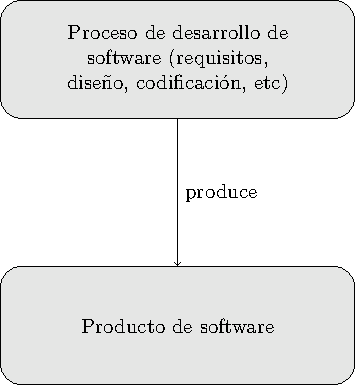
\includegraphics[width=0.4\textwidth]{image/cap2_img1.pdf}
\end{figure}
SQA se enfoca en el proceso. Se pregunta: ``¿Estamos construyendo el producto de la manera correcta?''

Testing se enfoca en el producto. Se pregunta: ``¿Hemos construido el producto correcto?''

\section{Medición y mejora de procesos}
Una famosa frase en el mundo de la gestión dice: 
``Lo que no se mide, no se puede mejorar''. 
Esta idea es el núcleo de este apartado del SWEBOK. 
Sin datos, cualquier intento de mejorar nuestros procesos de desarrollo de software se basa en la intuición, las corazonadas o, en el peor de los casos, en el azar. 
La medición nos proporciona el mapa y la brújula para navegar hacia procesos más eficientes y efectivos.

Imagina que eres el entrenador de un equipo deportivo. 
No te limitarías a decirles a tus jugadores ``¡sean mejores!''. 
Para mejorar de verdad, necesitarías medir su rendimiento:
\begin{itemize}
  \item ¿Cuál es el porcentaje de acierto en los tiros libres?
  \item ¿Cuántos kilómetros corren por partido?
  \item ¿Cuántos pases completan antes de perder el balón?
\end{itemize}

Solo con estos datos puedes identificar debilidades, probar nuevas estrategias (procesos) y medir si esas estrategias están funcionando. 
En la ingeniería de software, el principio es exactamente el mismo.

\subsection*{El Ciclo de la Mejora Continua}
El SWEBOK nos presenta la mejora de procesos no como un evento único, sino como un ciclo continuo y sostenible. 
Uno de los modelos más clásicos para ilustrar esto es el ciclo Planificar-Hacer-Verificar-Actuar (PDCA), también conocido como el ciclo de Deming.
Podemos visualizarlo de la siguiente manera:
\begin{figure}[H]
    \centering
    \caption{Ciclo de la mejora continua}
    \label{fig:ciclo_mejora_continua}
    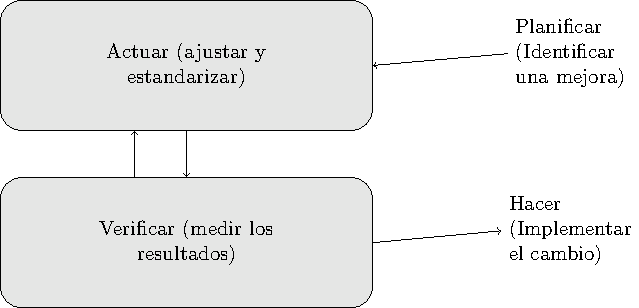
\includegraphics[width=0.6\textwidth]{image/cap2_img2.pdf}
\end{figure}
\begin{description}
  \item[Planificar (Plan):] ¿Qué queremos mejorar? El primer paso es identificar un área de mejora. Esto podría surgir del análisis de datos (por ejemplo, ``estamos encontrando demasiados errores durante las pruebas de sistema'') o de una nueva meta estratégica (``necesitamos reducir el tiempo de entrega en un 15\%''). Se define una hipótesis: ``Si implementamos revisiones de código formales, creemos que el número de errores encontrados en fases tardías disminuirá''.

  \item[Hacer (Do):] Implementar el cambio a pequeña escala. En lugar de cambiar la forma de trabajar de toda la organización de la noche a la mañana, se prueba el nuevo proceso en un entorno controlado. Por ejemplo, se introduce el proceso de revisión de código en un solo equipo o en un solo proyecto piloto.

  \item[Verificar (Check):] ¿Funcionó nuestra hipótesis? Aquí es donde la medición es crucial. Se recopilan datos del proyecto piloto y se comparan con los datos históricos (la línea de base). ¿Se redujo realmente el número de errores encontrados en las pruebas? ¿El esfuerzo extra en las revisiones de código se vio compensado por un menor esfuerzo en la depuración?

  \item[Actuar (Act):] Tomar una decisión basada en los datos. Si el nuevo proceso funcionó, se estandariza y se despliega a otros equipos o a toda la organización. Si no funcionó como se esperaba, se ajusta el proceso y se inicia el ciclo de nuevo con una nueva hipótesis. O quizás, se descarta la idea y se prueba otra diferente.
\end{description}

\chapter{Profesionalismo, ética y toma de decisiones}

\section{Profesionalismo, ética y responsabilidad legal}
El profesionalismo en ingeniería de software integra competencia técnica, conducta ética y cumplimiento legal. La práctica responsable exige no solo saber cómo diseñar y construir software, sino también entender el impacto social y legal de nuestras decisiones profesionales. En este sentido, \textcite{swebok2024} enfatiza que los códigos de conducta y los marcos regulatorios son elementos centrales para garantizar la confianza pública en los sistemas de software.

\begin{longtable}{p{3cm} p{12cm}}
\caption{Dimensiones del profesionalismo en ingeniería de software} \\
\toprule
\textbf{Dimensión} & \textbf{Descripción} \\
\midrule
\endfirsthead

\toprule
\textbf{Dimensión} & \textbf{Descripción} \\
\midrule
\endhead

\multicolumn{2}{r}{\textit{Continúa en la siguiente página}} \\
\endfoot

\bottomrule
\endlastfoot

Competencia técnica & Mantener y demostrar conocimientos actualizados (metodologías, lenguajes, prácticas de prueba y seguridad) y aplicarlos con juicio profesional. \\

Ética profesional & Actuar con integridad, transparencia y evitar conflictos de interés; reportar riesgos serios que puedan dañar a usuarios o terceros. \\

Responsabilidad legal & Cumplir leyes de propiedad intelectual, privacidad y regulaciones sectoriales; entender contractualidad y responsabilidad frente a fallos. \\

Impacto social & Evaluar consecuencias (sesgo, privacidad, seguridad) y diseñar mitigaciones para minimizar daños sociales. \\
\end{longtable}

\section{Dinámicas de grupo y habilidades de comunicación}
La ingeniería de software es esencialmente una actividad colectiva. El rendimiento del proyecto depende tanto de habilidades sociales (comunicación, liderazgo) como de capacidades técnicas.

\begin{longtable}{p{4cm} p{11cm}}
\caption{Dinámicas de grupo y su efecto en proyectos de software} \\
\toprule
\textbf{Dinámica} & \textbf{Efecto / uso en proyectos} \\
\midrule
\endfirsthead

\toprule
\textbf{Dinámica} & \textbf{Efecto / uso en proyectos} \\
\midrule
\endhead

\multicolumn{2}{r}{\textit{Continúa en la siguiente página}} \\
\endfoot

\bottomrule
\endlastfoot

Cooperativa & Facilita prácticas ágiles: planificación conjunta, revisiones de código y retroalimentación continua; reduce errores de integración y mejora la calidad. \\

Competitiva & Útil para innovación puntual (hackatones, concursos), pero si se mantiene sostenida puede fragmentar conocimiento y dificultar la colaboración. \\

Mixta & En organizaciones grandes, equipos colaboran internamente pero compiten por recursos; requiere coordinación, gobernanza y canales claros de transferencia de conocimiento. \\
\end{longtable}

\subsection*{Habilidades clave}
\begin{itemize}
  \item \textbf{Comunicación escrita:} documentación clara y concisa adaptada a distintos públicos.
  \item \textbf{Escucha activa:} comprender necesidades del cliente y del equipo para evitar malentendidos.
  \item \textbf{Presentación de resultados:} traducir lo técnico a lo no técnico y viceversa.
  \item \textbf{Resolución de conflictos:} negociar prioridades y compromisos sin sacrificar requisitos críticos.
\end{itemize}

\section{Fundamentos de economía y toma de decisiones}
Tomar decisiones informadas exige medir costos, beneficios y riesgos. El análisis económico aplicado al software ayuda a priorizar iniciativas y defender inversiones ante stakeholders.

\subsection*{Métricas económicas básicas}
\begin{itemize}
  \item \textbf{Costo total de propiedad (TCO):} suma de costos de desarrollo, operación y mantenimiento durante el ciclo de vida.
  \item \textbf{Retorno sobre la inversión (ROI):}
\end{itemize}

\begin{equation}\label{eq:roi}
ROI \;=\; \dfrac{\text{Beneficios proyectados} - \text{Costos de inversión}}{\text{Costos de inversión}}
\end{equation}
\noindent\textit{Ecuación \ref{eq:roi}. Cálculo del retorno sobre la inversión (ROI).}

\begin{itemize}
  \item \textbf{Valor Presente Neto (VPN):} evaluación de flujos de caja futuros descontados para decisiones multi-período.
\end{itemize}

\subsection*{Criterios de decisión}
Cuando hay múltiples alternativas, emplea criterios claros (valor esperado, ROI, TCO, impacto en plazo). Combinar métricas cuantitativas con juicios cualitativos (riesgo reputacional, cumplimiento legal) es práctica recomendable en proyectos críticos.

\section{Análisis de riesgo e incertidumbre}
Los riesgos en software pueden ser técnicos, de gestión o externos. Cuantificarlos y priorizarlos permite aplicar mitigaciones coste-efectivas.

\begin{longtable}{p{4cm} p{11cm}}
\caption{Clasificación breve de riesgos en proyectos de software} \\
\toprule
\textbf{Tipo de riesgo} & \textbf{Descripción / Ejemplo} \\
\midrule
\endfirsthead

\toprule
\textbf{Tipo de riesgo} & \textbf{Descripción / Ejemplo} \\
\midrule
\endhead

\multicolumn{2}{r}{\textit{Continúa en la siguiente página}} \\
\endfoot

\bottomrule
\endlastfoot

Técnico & Integración de tecnologías nuevas, deuda técnica que impide entregas puntuales, falta de pruebas automatizadas. \\

De gestión & Estimaciones erróneas, rotación de personal, dependencias externas incumplidas. \\

Externo & Cambios regulatorios, variaciones en el mercado, fallos de proveedores críticos. \\
\end{longtable}

\subsection*{Cuantificación rápida}
Un enfoque útil para priorizar riesgos es el Valor Esperado (EMV, Expected Monetary Value):

\begin{equation}\label{eq:emv}
EMV \;=\; \sum_{i} p_i \cdot c_i
\end{equation}
\noindent\textit{Ecuación \ref{eq:emv}. Valor Esperado (EMV) — probabilidad por impacto monetario para priorización de riesgos.}

La aplicación práctica del EMV requiere estimaciones conservadoras y revisión continua; sus fundamentos probabilísticos se apoyan en la literatura de estadística aplicada \parencite{ross2014}.

\subsection*{Estrategias de mitigación}
\begin{itemize}
  \item \textbf{Evitar:} cambiar el plan para eliminar riesgo crítico.
  \item \textbf{Transferir:} contratos, seguros y acuerdos SLA con penalidades claras.
  \item \textbf{Mitigar:} prototipos, pruebas tempranas, arquitecturas desacopladas y revisiones técnicas.
  \item \textbf{Aceptar:} asumir el riesgo cuando el costo de mitigación supera su impacto esperado.
\end{itemize}

\section{Análisis de compensación (trade-off analysis)}
El análisis de trade-offs permite comparar alternativas cuando los criterios son contradictorios (por ejemplo: rendimiento vs. costo, tiempo vs. calidad). Debe apoyarse en métricas medibles y, cuando proceda, en experimentación controlada.

\begin{longtable}{p{3cm} p{4cm} p{4cm} p{4cm}}
\caption{Ejemplo simplificado de análisis de compensación en arquitectura} \\
\toprule
\textbf{Alternativa} & \textbf{Ventaja principal} & \textbf{Desventaja} & \textbf{Adecuado para} \\
\midrule
\endfirsthead

\toprule
\textbf{Alternativa} & \textbf{Ventaja principal} & \textbf{Desventaja} & \textbf{Adecuado para} \\
\midrule
\endhead

\multicolumn{4}{r}{\textit{Continúa en la siguiente página}} \\
\endfoot

\bottomrule
\endlastfoot

Monolito & Simplicidad de despliegue y menor sobrecarga operacional & Escalabilidad y despliegue restringidos; acoplamiento elevado entre módulos & Proyectos pequeños / POC \\

Microservicios & Escalabilidad independiente y despliegue por servicio & Complejidad en orquestación, observabilidad e integración & Sistemas grandes, equipos distribuidos \\

Serverless & Baja inversión inicial y facturación por uso & Dependencia del proveedor y límites de ejecución & Prototipos, cargas variables y validaciones rápidas \\
\end{longtable}

\subsection*{Notas sobre trade-offs algorítmicos}
En elecciones algorítmicas o de diseño interno, la literatura clásica enfatiza que mejorar una métrica normalmente perjudica otra (por ejemplo, tiempo vs. espacio). Para decisiones de este tipo, apóyate en análisis de complejidad y medidas empíricas antes de optar por una solución \parencite{clrs2009,knuth1997}.


\chapter{Fundamentos técnicos relacionados}
\label{chap:fundamentos}

La Ingeniería de Software, como disciplina, requiere un entramado sólido de conocimientos técnicos complejos que apoyen la elaboración, evaluación y evolución de sistemas informáticos efectivos y confiables. Este capítulo pretende ofrecer una visión ampliada y profunda de los fundamentos técnicos claves involucrados, en línea con los estándares y prácticas recomendadas en el \textit{Software Engineering Body of Knowledge (SWEBOK)} \parencite{swebok2024}. Los conceptos abordados aquí habilitan a los ingenieros a tomar decisiones fundamentadas y efectuar análisis rigurosos en proyectos complejos.

\section{Fundamentos de computación: Algoritmos y estructuras de datos}
Los algoritmos y estructuras de datos constituyen el corazón del diseño y evaluación del software eficiente. Más allá de la simple implementación de funciones, comprender el impacto temporal y espacial de las soluciones permite diseñar sistemas con desempeño predecible y optimizado. Además, la elección adecuada de estructuras —como listas enlazadas, árboles balanceados o tablas hash— influye decisivamente en la escalabilidad.

Este conocimiento se articula no solo en la corrección funcional, sino en el análisis formal mediante notaciones asintóticas ($O(\cdot)$, $\Theta(\cdot)$, $\Omega(\cdot)$) que describen límites inferiores y superiores para el uso de recursos computacionales \parencite{clrs2009,knuth1997}. Técnicas modernas incluyen estrategias de programación dinámica, algoritmos voraces y paradigmas de divide y vencerás, necesarios antes de afrontar la complejidad inherente a problemas reales.

\subsection*{Temas esenciales}
\begin{itemize}
  \item Verificación formal de algoritmos: pruebas mediante invariantes y métodos inductivos.
  \item Complejidad computacional: clasificación y comparación de algoritmos para decisión informada.
  \item Estructuras avanzadas: montículos para colas de prioridad, grafos para modelado de relaciones complejas.
  \item Aplicaciones: algoritmos clásicos como Dijkstra para rutas, Kruskal para árboles de expansión mínima, algoritmos de búsqueda en profundidad y amplitud.
  \item Consideraciones en ingeniería: coste amortizado, optimización para jerarquías de memoria, y diseño concurrente.
\end{itemize}


\section{Fundamentos matemáticos: Lógica y probabilidad discreta}
La base matemática que sustenta la ingeniería de software permite formalizar el razonamiento con precisión. La lógica proposicional y de primer orden es el lenguaje para especificaciones y verificación automatizada de sistemas, garantizando corrección y comportamiento deseado. Por otra parte, la teoría de conjuntos y combinatoria estructuran la resolución de problemas discretos, mientras que la teoría de grafos modela relaciones y flujos de información intrínsecos a muchas arquitecturas software \parencite{rosen2019,ross2014}.

La probabilidad discreta provee herramientas para enfrentar la incertidumbre y analizar algoritmos aleatorizados, además de ser fundamental para el análisis estadístico aplicado en evaluación y predicción del comportamiento del software.

\subsection*{Temas esenciales}
\begin{itemize}
  \item Lógica formal y métodos de deducción automática.
  \item Técnicas combinatorias y principios de conteo para análisis exhaustivos.
  \item Propiedades y algoritmos en grafos: conectividad, recorridos, y coloración.
  \item Probabilidad discreta: variables aleatorias, esperanza matemática, varianza y distribuciones relevantes.
  \item Modelos probabilísticos aplicados, como cadenas de Markov para sistemas estocásticos.
\end{itemize}


\section{Fundamentos de ingeniería: Modelado y análisis estadístico}
El enfoque empírico en ingeniería de software demanda la transformación de datos observados en conclusiones válidas mediante el modelado estadístico. Aspectos críticos incluyen la estimación de parámetros de desempeño y calidad, pruebas de hipótesis para validar supuestos, y análisis de confiabilidad para prever la tasa y naturaleza de fallos \parencite{ross2014,swebok2024}.

Las prácticas instrumentales como el diseño experimental y la validación cruzada son imprescindibles para obtener resultados confiables y generalizables, sentando bases para decisiones informadas y mejoras continuas en procesos y productos.

\subsection*{Temas esenciales}
\begin{itemize}
  \item Diseño experimental robusto y cálculo del tamaño muestral adecuado para asegurar representatividad.
  \item Técnicas de estimación puntual y por intervalos, con aplicación de pruebas paramétricas y no paramétricas.
  \item Modelos predictivos mediante regresión y clasificación; implementación y evaluación mediante validación cruzada.
  \item Métricas de confiabilidad y análisis de modelos de tasas de fallo para anticipar y mitigar riesgos.
\end{itemize}


\section{Organización de computadoras y sistemas operativos}
El conocimiento de la arquitectura informática y sistemas operativos provee la comprensión necesaria para mejorar el rendimiento y la seguridad del software. Desde la jerarquía de memoria, donde intervienen registros, caché y memoria principal, hasta la gestión de procesos y mecanismos de entrada/salida, cada capa influye en la ejecución y estabilidad del sistema \parencite{patterson2014,tanenbaum2014}.

Este entendimiento es vital para optimizar la asignación de recursos, coordinar concurrencia y evitar condiciones problemáticas como deadlocks, aspectos imprescindibles en el desarrollo profesional riguroso.

\subsection*{Temas esenciales}
\begin{itemize}
  \item Unidades de procesamiento y modelos de memoria.
  \item Estructura y funcionamiento de la jerarquía memoria-caché-registros.
  \item Gestión de procesos, sincronización, exclusión mutua y prevención de bloqueos.
  \item Algoritmos y políticas para planificación de CPU, paginación, swapping, y virtualización.
  \item Arquitectura de dispositivos y manejo seguro de E/S.
\end{itemize}


\section{Conceptos de redes y bases de datos}
Las redes y bases de datos constituyen los pilares para la construcción de sistemas distribuidos y aplicaciones empresariales modernas. Es fundamental comprender el modelo OSI/TCP-IP, protocolos de transporte y seguridad para garantizar comunicaciones confiables y seguras \parencite{silberschatz2010,swebok2024}.

En el ámbito de bases de datos, el modelado conceptual, normalización adecuada, gestión de transacciones y optimización de consultas forman el núcleo para la integridad y eficiencia de los datos almacenados y procesados.

\subsection*{Temas esenciales}
\begin{itemize}
  \item Modelos de referencia para redes y pila de protocolos (OSI/TCP-IP).
  \item Protocolos fundamentales: IP, TCP, UDP, y variantes HTTP/2/3, incluyendo mecanismos de seguridad TLS.
  \item Diseño y normalización de bases de datos relacionales, gestión ACID, índices y técnicas de optimización.
  \item Sistemas distribuidos: modelos de consistencia, tolerancia a fallos y patrones de diseño como consenso y elección de líder.
\end{itemize}


\section*{Cierre del capítulo}
Este capítulo ha desarrollado un marco técnico integral que sirve como base para el análisis, diseño y mejora de procesos y productos en ingeniería de software, en concordancia con el SWEBOK. La integración de fundamentos computacionales, matemáticos, estadísticos e infraestructurales es condición necesaria para abordar con efectividad los retos actuales en testing y calidad del software, tarea que continúa en los siguientes capítulos de este trabajo.

\chapter*{CONCLUSIONES}
\label{cap:conclusiones}
\addcontentsline{toc}{chapter}{Conclusiones}

A lo largo de este trabajo se ha explorado la ingeniería de software a través de la perspectiva del SWEBOK, entendido como una guía que orienta la construcción de sistemas confiables y sostenibles. Más que un compendio de prácticas, constituye una brújula que acompaña el ciclo de vida del software, desde la concepción de una idea hasta el mantenimiento que asegura su vigencia en el tiempo.

El análisis de requisitos resaltó la necesidad de un entendimiento claro con los interesados para evitar inconsistencias en el producto final. El diseño arquitectónico reafirmó la importancia de una base sólida y flexible, capaz de adaptarse a cambios futuros. La construcción y codificación mostraron que el código no solo debe ser funcional, sino también comprensible y mantenible.

Las pruebas fueron concebidas como un mecanismo sistemático para identificar fallos y garantizar la calidad, mientras que el mantenimiento se presentó como un proceso continuo y fundamental para la evolución del software, considerando sus dimensiones correctiva, adaptativa, perfectiva y preventiva.

En los procesos, la gestión de configuración se destacó como pilar para el control de versiones y la trazabilidad. La planificación y el seguimiento se identificaron como prácticas esenciales para alinear esfuerzos, mientras que los modelos de ciclo de vida, tanto predictivos como adaptativos, evidenciaron la necesidad de ajustar la estrategia a las características del proyecto. El aseguramiento de la calidad y la medición se establecieron como bases para la mejora continua.

El estudio también subrayó el rol del profesionalismo y la ética en la toma de decisiones, considerando riesgos y compensaciones necesarias para mantener la responsabilidad en la práctica. Asimismo, los fundamentos técnicos en algoritmos, lógica, estadística, hardware y redes fueron reconocidos como el soporte esencial que posibilita la implementación de las prácticas descritas.

En síntesis, el SWEBOK no debe interpretarse únicamente como un marco de referencia, sino como una invitación a aplicar sus principios en proyectos reales, fomentando la construcción de software eficiente, sostenible y valioso para la sociedad.


\printbibliography

\end{document}
